\vspace{-20pt}

\subsection*{主要学术成绩概述}

凝聚态体系中的\emph{激发态动力学}是决定凝聚态物质性质的关键,从时间、空间、能量、
动量、自旋等多个维度来理解乃至于调控凝聚态体系的超快动力学过程是现代凝聚态物理重
要的新兴方向之一。申请人自\emphNum{2016}年到中国科大工作以来,\emph{聚焦凝聚态体
  系激发态动力学的理论和应用研究},取得了一系列重要的进展和成果,包括:

\begin{enumerate}
[
  leftmargin=15pt
]
\kaishu{}
  
\item \emph{发展和推广}第一性原理激发态动力学程序包\hnamd{}。该软件包是一个具有独
  立知识产权、自主可控的激发态动力学第一性原理计算软件,旨在对激发态载流子动力学
  进行研究,聚焦于电子空穴的复合、界面超快电荷转移、谷电子和谷激子动力学、动量空
  间载流子动力学等问题,在光电器件以及清洁能源材料等领域有重要的应用。申请人贡献
  了该程序的\emph{初版的主要代码和框架,并指导增加后续其他功能},比如\emph{率先实
    现了自旋分辨的$GW+{}$rtBSE方法},突破了$GW+{}$BSE 方法在含时动力学上的瓶颈,
  使固体激发态动力学可以准确包含激子多体效应;实现了\emph{动量空间实时载流子动力
    学模拟(\namdk)},需要利用单胞计算电声耦合即可,\emph{大幅降低}了计算量,为
  研究材料中的载流子在动量空间中的动力学行为提供了有力的工具,也为研究光致相变、
  光催化提供了可能的技术手段。
  
\item 利用\hnamd{}系统地研究了一系列\emph{固体材料中的激发态动力学问题}:
  \begin{enumerate*} [label=\textnormal{(\roman*)}]
    
  \item 研究了不同\emph{界面体系激发态电荷的转移}的动力学过程,阐明界面激发态电子、
    声子等准粒子相互耦合的复杂超快过程中的物理机制;

  \item 定量研究了半导体材料中的\emph{电子空穴复合}中心的形成机制,为设计高效率的
    光电器件材料做出了理论预言;
    
  \item 研究了一系列\emph{表面吸附单分子激发态动力学},为单分子激发态动力学提供了
    时间、空间和能量等多个维度的物理图像。
  \end{enumerate*}
\end{enumerate}

申请人计划未来继续专注于凝聚态体系激发态动力学,xxxx,揭示新兴量子材料中激发态动
力学的物理机制,力争解决更多凝聚态领域激发态动力学的重要科学难题。

%%%%%%%%%%%%%%%%%%%%%%%%%%%%%%%%%%%%%%%%%%%%%%%%%%%%%%%%%%%%%%%%%%%%%%%%%%%%%%%%
% 共发表文章52篇,其中在【Frontiers of Data and Computing】、【Fundamental
% Research】和【Electronic Structure】上发表的3篇属于ESCI收录。
%%%%%%%%%%%%%%%%%%%%%%%%%%%%%%%%%%%%%%%%%%%%%%%%%%%%%%%%%%%%%%%%%%%%%%%%%%%%%%%%

申请人共发表SCI/ESCI收录文章\emphNum{52}篇,% \emph
{
  近五年共发表论文\emphNum{38}篇,
  其中以(共同)通讯/(共同)第一作者发表
  \emphNum{1}篇{\itshape Nat.\ Comp.\ Sci.}、
  \emphNum{1}篇综述性文章{\itshape WIRES Comput.\ Mol.\ Sci.}、
  \emphNum{2}篇{\itshape Phys.\ Rev.\ B}、
  \emphNum{1}篇{\itshape Nano Lett.}、
  \emphNum{5}篇{\itshape J.\ Phys.\ Chem.\ Lett.},
  全部文章总引用次数\emphNum{2029}次,H因子\emphNum{26}(Google Scholar 数据)。
}

%%%%%%%%%%%%%%%%%%%%%%%%%%%%%%%%%%%%%%%%%%%%%%%%%%%%%%%%%%%%%%%%%%%%%%%%%%%%%%%%
\subsection*{一、发展和推广了第一性原理计算激发态动力学程序\hnamd{}}
%%%%%%%%%%%%%%%%%%%%%%%%%%%%%%%%%%%%%%%%%%%%%%%%%%%%%%%%%%%%%%%%%%%%%%%%%%%%%%%%

\begin{center}
  \begin{InnovationBox}
    贡献了自主知识产权的第一性原理激发态动力学程序\hnamd{}的主要代码和框架,并指
    导增加后续其他功能:首次实现了自旋分辨$GW+{}$rtBSE方法,用于研究自旋分辨激子动力
    学,准确包含多体效应;实现了动量空间实时载流子动力学模拟,大幅降低计算量等。
    同时致力于\hnamd{}的推广,程序已得到越来越多的应用。
  \end{InnovationBox}
\end{center}

%%%%%%%%%%%%%%%%%%%%%%%%%%%%%%%%%%%%%%%%%%%%%%%%%%%%%%%%%%%%

第一性原理(first-principles)计算是人们理解凝聚态物质本质的重要工具,传统的第一
性原理计算基于玻恩--奥本海默近似,关注材料基态的电子结构,可以得到不同原子核的相
互作用势,从而进行基态的分子动力学计算。然而,\emph{考虑到激发态下的晶格、电子、
  自旋动力学,目前并没有成熟的第一性原理计算方法与软件,这也是第一性原理计算发展
  的新方向}。总得来说,激发态动力学模拟的基本思路是将不同层次的电子结构方法,例如
密度泛函理论、 线性响应含时密度泛函、$GW+{}$BSE等,与动力学的一些方法,例如含时薛定谔
方程、含时科恩-沈吕九方程、平均场动力学、轨迹面跳跃以及分子动力学等方法相结合,来
研究晶格、电子、自旋的动力学过程。

激发态弛豫的过程实际上描述的是与原子核运动耦合在一起的电子在不同本征态之间跃迁的
过程,由于\emph{涉及到不止一个势能面},这类问题显然是\emph{超越玻恩--奥本海默近
  似}的。在化学动力学领域,包含非绝热效应的动力学方法有很长的发展历史,对于模型体
系或原子数非常少的小分子体系,可以用所谓“全量子”方法,也就是将原子核与电子都当成
量子粒子来处理。然而,\emph{全量子方法的计算量非常大},\emph{无法处理凝聚态材料体
  系这种复杂体系}。因此,人们往往使用\emph{混合量子-经典}的非绝热动力学方法,把原
子核当成经典粒子、电子当成量子粒子来分开处理。这其中主要的思路有两类,一类是与平
均场动力学方法相结合,在平均场势能面上同时演化原子核与电子,基于这个思路发展的方
法其实就是实时的含时密度泛函方法。另一类被笼统地称作NAMD方法,这里人们将实时演化
的科恩--沈方程与面跳跃方法相结合,引入经典路径近似,利用分子动力学得到晶格演化的
实时轨迹,以此来模拟声子的激发,然后在此基础上模拟载流子的弛豫过程。这种方法最早
由美国南加州大学Oleg V. Prezhdo教授提出,并应用于固体体系。他与纽约州立大学水牛城
分校的A. Akimov教授共同发展了PYXAID程序,可以在单粒子图像下模拟电子或空穴的动力学
过程。\emph{在这个理论框架的基础上,申请人所在中国科学技术大学的赵瑾教授研究组发
  展了\hnamd{}(\url{https://hefei-namd.org/})程序,并用来模拟界面电荷转移、电子
  空穴复合等动力学过程,申请人贡献了该程序的最初版本的主要代码和框架}。

近年来,以过渡金属硫族化合物、黑磷等为代表的二维材料,由于其丰富的光学激发态和诸
多超越传统体材料的物理性质,受到了研究者的普遍关注和重视。其中,二维材料中量子限
域效应导致库伦作用并不能被有效屏蔽,电子空穴间的库伦作用比较强,由此产生了各种各
样有意思的多体效应,比如形成各种各样的激子:亮激子、暗激子、谷激子和层间激子等。
针对这个问题,2021年我们将单体的实时科恩--沈方程替换为两体实时BSE方程,
在\hnamd{}中实现了$GW{}+{}$rtBSE--NAMD方法,进一步引入了自旋轨道耦合,可以用来研
究光激发之后的自旋分辨激子弛豫动力学,\emph{文章发表在\textit{Sci.\ Adv.}上,申请
  人在其中起了重要的作用}。


在传统的NAMD框架下研究具有周期性边界条件的固体,人们常常使用\emph{超胞
  法}和\emph{分子动力学}来模拟固体中声子的激发。由于使用了周期性边界条件,只有超
胞的$\Gamma$点的声子才会被激发,而超胞$\Gamma$点的声子又是由单胞中某些满
足\emph{折叠条件}的声子折叠过去的。这就导致了使用该方法模拟所包含的电声散射中涉及
到电子动量$\mathbf{k}$和声子动量$\mathbf{q}$点\emph{受到超胞大小的限制},对于电子
和声子色散比较强的体系会产生较大的困难。为了解决这个问题,2023年申请人所在研究团
队在\hnamd{}中将电声耦合矩阵元引入含时演化哈密顿量,实现了动量空间的非绝热动力
学(\namdk{})方法。他们用这种方法研究了石墨烯体系的热电子弛豫过程,与实验得到了较
为一致的结果。\emph{文章发表在2023年的\textit{Nat.\ Comp.  Sci.}上,申请人为共同
  通讯作者}。与此几乎同时,上海科技大学的郑帆教授与半导体所的汪林望研究员通过引入
声子的平带近似,也实现了一种多$\mathbf{k}$点的NAMD方法。


\begin{figure}
  \centering
  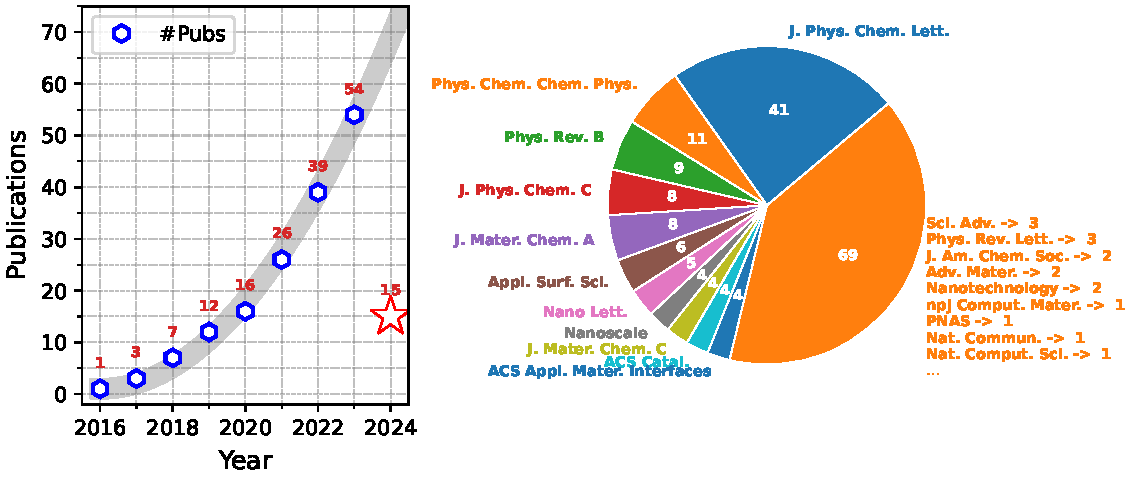
\includegraphics[width=1.0\linewidth]{figs/hefei-namd_pub_v3.pdf}
  \caption{\label{fig:hnamd_pub_list}
    \kaishu{}\footnotesize
    (左)自2016年起,历年使用\hnamd{}发表的文章数,其中2024年度截止二月份已
    发表\emphNum{15}篇文章。
    (右)使用\hnamd{}发表文章的期刊组成图。
  }
\end{figure}


在发展程序的同时,\emph{申请人还致力于程序的推广},2018至2023年在“凝聚态物质激发
态研讨会”上进行了\emphNum{5}次规模在\emphNum{100}人左右的软件培训。至今为
止,\hnamd{}的用户包括美国科学院院士 Shaul Mukamel、澳大利亚科学院院士 Shixue
Dou、爱荷华州立大学的Kaiming Ho、伦敦皇家学院的 Aron Walsh、卡内基梅隆大学的 Noa
Marom、纽约州立大学的 A. Akimov、中国科学技术大学杨金龙院士、东南大学王金兰教授、
华南师范大学赵纪军教授(原就职于大连理工大学)、山东大学赵明文教授等数十个研究
组。
% 例如,东南大学王金兰课题组用来计算异质结电子空穴分离与复合的效率,由此设计Z型光
% 催化材料 [\textit{ACS Catalysis} 20, 1976 (2020)];中国科学技术大学的朱彦武教授
% 用来研究双层石墨烯热电子弛豫与声子的耦合 [\textit{Phys.  Rev. Lett.}, 126,
% 027402 (2021)]等。
从 {\large{}2016} 年起,本领域使用\hnamd{}发表的文章数目逐年增加,如
图-\ref{fig:hnamd_pub_list}所示。\emph{截止2024年2月,基于 \hnamd{} 发表论文总数
  已高达 \emphNum{173} 篇},其中不乏括 \textit{Phys. Rev.  Lett.},\textit{Nat.
  Commun.},\textit{Sci.  Adv.},\textit{npj Comput.
  Mater.},\textit{Phys. Rev.  B},\textit{PNAS},\textit{JACS},\textit{JPCL}等
在内的的高水平期刊。图-\ref{fig:hnamd_pub_list}列举了历年利用\hnamd{}发表的文章数,
以及发表文章的期刊组成,发表文章详细信息参见\textbf{附录1.1}。申请人相信,通过持
续的努力,比能将 \hnamd{} 发展成为源于国内、独立知识产权、自主可控、并拥有重要国
际影响力的第一性原理激发态动力学程序。

%%%%%%%%%%%%%%%%%%%%%%%%%%%%%%%%%%%%%%%%%%%%%%%%%%%%%%%%%%%%%%%%%%%%%%%%%%%%%%%%
\subsection*{二、研究了不同固体材料激发态载流子动力学}
%%%%%%%%%%%%%%%%%%%%%%%%%%%%%%%%%%%%%%%%%%%%%%%%%%%%%%%%%%%%%%%%%%%%%%%%%%%%%%%%
\begin{center}
  \begin{InnovationBox}
    研究了不同固体材料中的激发态载流子动力学,包括:提出了范德华异质结界面声子辅
    助超快电荷转移的机理;揭示了分子振动激发对热电子捕获的关键影响;提出硬度较低
    的半导体材料不易形成电子空穴复合中心的理论预言;研究了一系列表面吸附单分子激
    发态动力学,为单分子激发态动力学提供了时间、空间和能量等多个维度的物理图像。
  \end{InnovationBox}
\end{center}

\begin{figure}
  \centering
  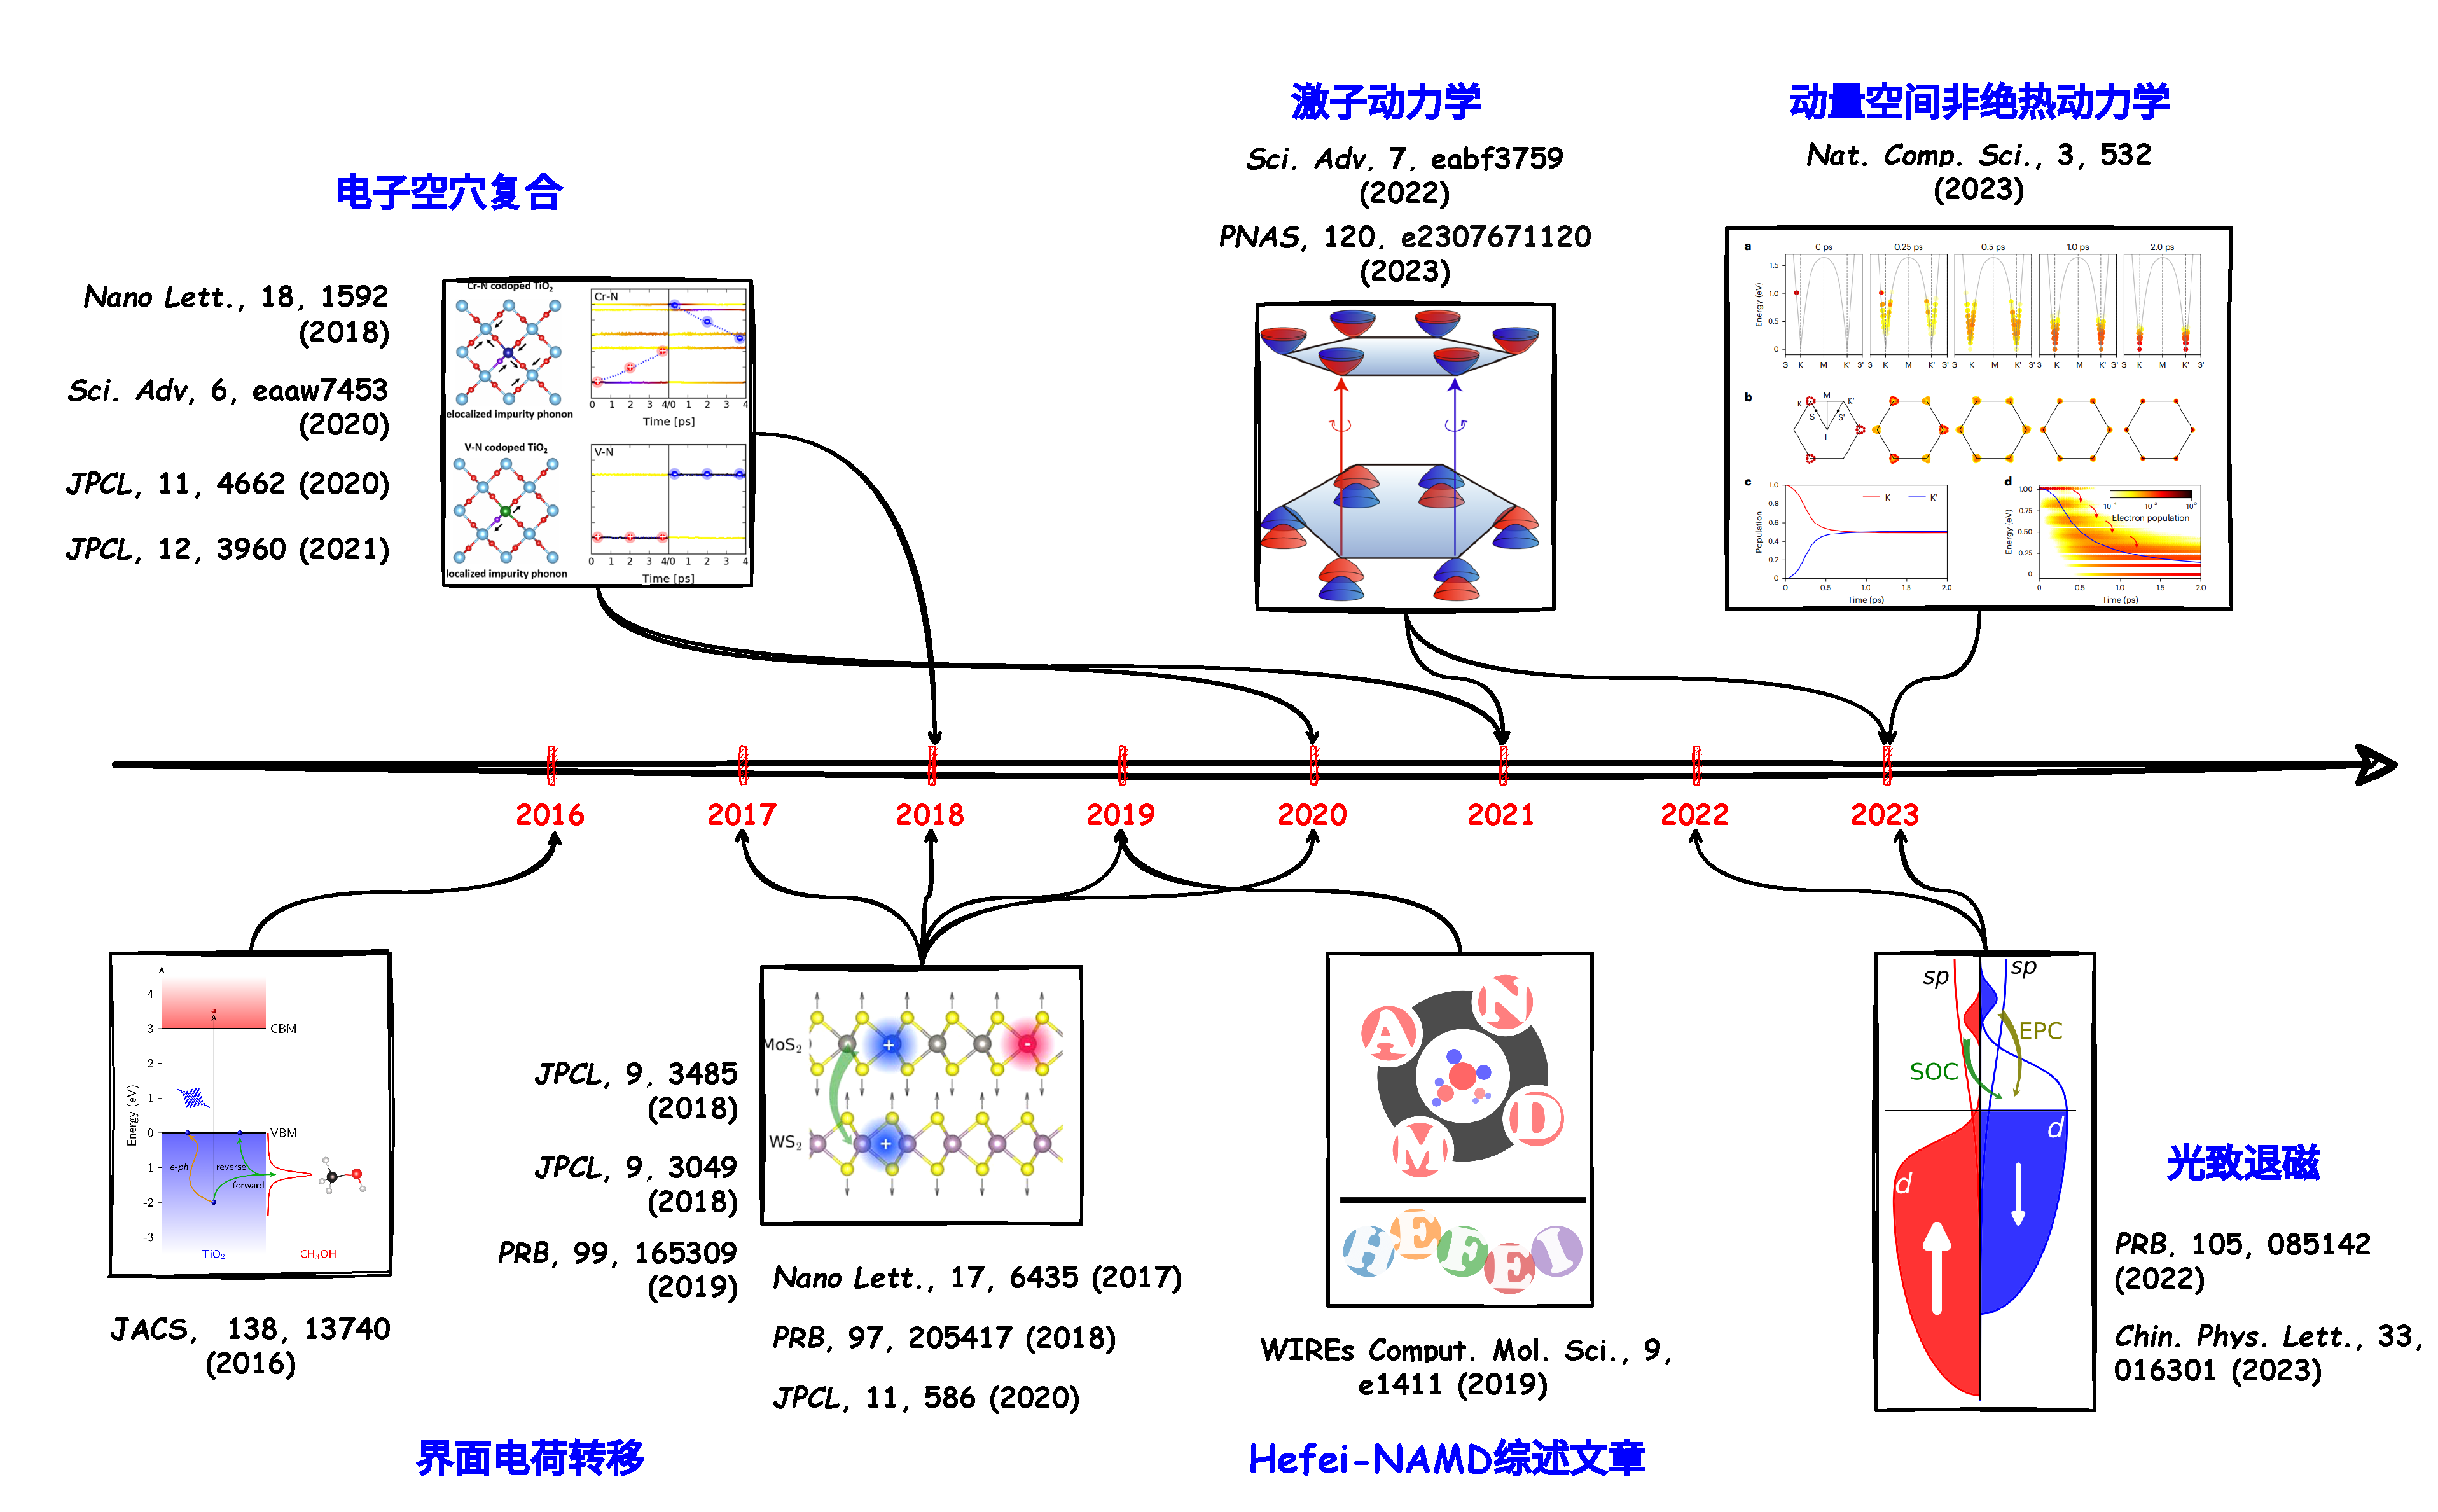
\includegraphics[width=1.\linewidth]{figs/rep_work.pdf}
  \caption{\label{fig:fig_rep_work}
    \kaishu{}\footnotesize
    申请人历年利用Hefei-NAMD做出的一些重要工作总结。
  }
\end{figure}


固体材料中的激发态载流子动力学是影响光电及能源器件效率的关键之一。在太阳能电池、
光电器件、表面等离激元以及光催化等领域,激发态载流子的动力学行为决定了材料与器件
的效率,理解了激发态动力学行为,才有可能解决能源材料与器件领域的重要问题。申请人
分别在界面电荷转移、半导体电子空穴复合以及表面分子激发态等方向取得了一系列成就,
成果总结于图-\ref{fig:fig_rep_work}中,现就其中几点重点展开:

%%%%%%%%%%%%%%%%%%%%%%%%%%%%%%%%%%%%%%%%%%%%%%%%%%%%%%%%%%%%%%%%%%%%%%%%%%%%%%%%
\subsubsection*{\rom{1})提出范德华异质结超快界面电荷转移物理机制}
%%%%%%%%%%%%%%%%%%%%%%%%%%%%%%%%%%%%%%%%%%%%%%%%%%%%%%%%%%%%%%%%%%%%%%%%%%%%%%%%

% \begin{enumerate}[label=\textnormal{\color{EmphColor}\Roman*.}]
% \item {\color{EmphColor}\kaishu\bfseries{}
%     提出范德华异质结、金属纳米颗粒/半导体超快界面电荷转移物理机制
% }


%   Nano Lett., 17, 6435 (2017)
% https://webofscience.clarivate.cn/wos/woscc/full-record/WOS:000413057500080   

在二维材料兴起之后,范德华异质结材料由于其在光电器件领域的潜力受到了人们大量的关
注,这类界面相互作用很弱,不存在化学键,但多个实验组都证明界面存在时间尺度在数十
飞秒的超快电荷转移,这其中的物理机制人们还无法理解。我们利用 \hnamd{} 研究了过渡
金属硫族化物(TMD)界面的电荷转移过程,发现电声耦合在界面电荷转移中起到了非常重要
的作用,在 MoS$_2$/WS$_2$ 界面,光学支声子的辅助是空穴超快转移的重要原
因[\textit{Nano Lett.} 17, 6435 (2017)](代表性工作 2,引
用\emphNum{196}次),在 MoSe$_2$/WSe$_2$ 界面,由于更强的电声耦合,甚至会发生声子
耦合的界面电荷振荡[\textit{Phys.\ Rev.\ B}, 97, 205417 (2018)]。我们还进一步提出
可以通过施加应力的方法调控界面电荷转移的时间尺度[\textit{J.\ Phys.\ Chem.\
  Lett.}, 11, 586 (2020)];这些工作成功地揭示了声子激发以及电声耦合在界面电荷转移
动力学中的重要作用。

\begin{justify} 
  %%%%%%%%%%%%%%%%%%%%%%%%%%%%%%%%%%%%%%%%%%%%%%%%%%%%%%%%%%%%%%%%%%%%%%%%%%%%%%%%
  \small\kaishu\color{magenta}{}
  %%%%%%%%%%%%%%%%%%%%%%%%%%%%%%%%%%%%%%%%%%%%%%%%%%%%%%%%%%%%%%%%%%%%%%%%%%%%%%%%
  我们提出的声子辅助电荷转移的机制被哥伦比亚大学 Howard Family 教授 X.Y.  Zhu的时
  间分辨超快实验证实,他们直接观察到了电荷转移与声子的耦合[\textit{Phys.\ Rev.\
    B}, 101, 201405 (2020)], 声子辅助超快电荷转移这一概念也被广泛接受,德国巴伐利
  亚科学院院士 U.  H\"ofer 教授[\textit{Phys. Rev. B}, 102, 125417(2020),
  \textit{Nanoscale}, 5, 1603 (2020)],德国马普所
  的 Gierz 教授[\textit{Sci. Adv.}, 6, eaay0761 (2020)], 及浙江大学的朱海明教
  授[\textit{J. Phys. Chem. Lett.}, 10, 150 (2019)] 用我们提出的概念成功地解释了
  他们的实验结果(附录 2.1-2.5)。2019 年被 Web of Science 评为诺奖热门人选的斯坦
  福大学Tony Heinz 教授在其发表在\textit{Nat. Nanotech.}上的综述中评价到:“最近一
  些工作证实了声子在电荷转移中的直接作用\ldots{}人们认为声子可以将电子从K谷散射
  搞$\Gamma$谷,此时层间有更强的杂化,有助于电荷转移的发生\ldots{}Zheng等人利
  用TDDFT方法证实了这个原理。”[\textit{Nat.\ Nanotech.}, 57, 5320
  (2018)](附录2.6)。
\end{justify}

  
% \item {\color{EmphColor}\kaishu\bfseries{}
%     发现电子空穴复合中心的产生与半导体硬度的关系,提出调控载流子寿命的理论方案
%   }

\subsubsection*{\rom{2})半导体中电子空穴复合动力学}

半导体材料常有的缺陷和杂质会产生电子空穴复合中心,降低器件的效率,如何通过材料设
计尽量减少半导体材料的电子空穴复合中心是这个领域的重要问题。我们研究了一系列半导
体材料中的电子空穴复合动力学,在 TiO$_2$ 为代表的氧化物半导体中,我们发现能量位于
能隙中间的深杂质能级会成为电子空穴复合中心,这与人们熟悉的 Shockley-Reed-Hall
(SRH) 模型给出的结论一致[\textit{Nano Lett.}, 18, 1592, (2018)]。然而,在有机钙钛
矿太阳能电池(MAPbI$_3$)的工作中,我们却发现无论是深能级缺陷还是浅能级缺陷,都没
有形成明显的电子空穴复合中心,分析表明主要原因是由于这种材料硬度很低,因此导带底、
价带顶与缺陷能级都只与低频声子耦合,从而使得无论缺陷是深能级还是浅能级,电子空穴
复合都很慢,不会有复合中心的形成。因此,我们提出硬度较低的半导体材料不易形成电子
空穴复合中心,这类材料可能在清洁能源及光电器件方面有重要的应
用 [\textit{Sci. Adv.}, 6, eaaw7453, (2020)]上。

\begin{justify}
  %%%%%%%%%%%%%%%%%%%%%%%%%%%%%%%%%%%%%%%%%%%%%%%%%%%%%%%%%%%%%%%%%%%%%%%%%%%%%%%%
  \small\kaishu\color{magenta}{}
  %%%%%%%%%%%%%%%%%%%%%%%%%%%%%%%%%%%%%%%%%%%%%%%%%%%%%%%%%%%%%%%%%%%%%%%%%%%%%%%%
  文章发表后引起了业内同行的关注,苏黎世理工大学的 KovalenKo 教授用我们提出的概念
  解释了他们的 NMR 和 NQR 实验(JACS 2020)北京师范大学的方维海院士在他们的文章中
  用详细介绍了我们在电子空穴复合方面的工作 (JMCA 2020): “Zhao 与合作者研究了不同
  材料中的电子空穴复合动力学,包括钙钛矿、金红石TiO$_2$、黑磷等,为设计高效光伏和
  光催化材料提供了重要的理论依据\ldots{}”[附录 5.1-5.2]
\end{justify}


\subsubsection*{\rom{3})表面吸附单分子激发态动力学}

表面分子对激发态电子空穴的捕获过程是分子光电器件的关键过程,我们利用 \hnamd{} 成
功地给出了表面单分子激发态动力学在时间、空间、能量等多个维度上的物理图像。
在 CH$_3$OH/TiO$_2$ 体系中,我们发现只有解离的 CH$_3$O 才有较强的捕获激发态空穴的
能力,捕获空穴的时间尺度约为 150 飞秒,空穴被CH$_3$O 捕获之后,其中一部分会在 10
飞秒之后重新回到 TiO$_2$,发生反向空穴转移,而分子的振动会加快 TiO$_2$ 内部热空穴
向价带顶的弛豫。在这个动力学过程中,分子-固体的能级匹配、声子的激发及电声耦合的大
小是决定分子捕获空穴20的关键因素。[\textit{J. Am. Chem. Soc.}, 138, 13740
(2016)] 而 TiO$_2$ 表面 CO$_2$ 分子的弯曲和非对称拉伸两种振动模式如果能够被有效激
发,CO$_2$ 的 LUMO 轨道则会被降低至导带底之下,并保持 150 飞秒左右的时间,此
时 CO$_2$ 可以在 80 飞秒之内有效捕获导带上的电子,并在之后的 30--40 飞秒 发生解离
形成 CO 分子。这项工作揭示了CO$_2$ 振动模式激发在光还原过程中的关键性作用,并从第
一性原理计算的角度对TiO$_2$ 表面 CO$_2$ 分子的光致还原的激发态动力学给出了清晰的
描述。[\textit{J. Am. Chem.  Soc.}, 142, 3214, (2020) - 代表性工作 5)]。
  
\begin{justify}
  %%%%%%%%%%%%%%%%%%%%%%%%%%%%%%%%%%%%%%%%%%%%%%%%%%%%%%%%%%%%%%%%%%%%%%%%%%%%%%%%
  \small\kaishu\color{magenta}{}
  %%%%%%%%%%%%%%%%%%%%%%%%%%%%%%%%%%%%%%%%%%%%%%%%%%%%%%%%%%%%%%%%%%%%%%%%%%%%%%%%
  针对CH$_{3}$OH/TiO$_{2}$的工作,中国科学技术大学的张群教授与罗毅教授针对这项工
  作专门设计了时间分辨的超快光谱学实验,来研究CH$_{3}$OH/C$_{3}$N$_{4}$界面的空穴
  捕获动力学[\textit{Angew. Chem. Int. Ed.}, 57, 5320, (2018)]。他们在文章引言部
  分用一整段来描述实验动机:“最近,Chu等人提出了CH$_{3}$OH/TiO$_{2}$界面电荷转移
  的物理图像…考虑到半导体界面空穴转移动力学的独特性质,用实验来验证理论的预测是非
  常关键的。”他们的实验验证了我们文中的主要结论: i)只有 CH$_{3}$O 可以捕获空
  穴;ii)存在反向空穴转移的过程(附件 4.8)。杨学明院士的双光子光电子能谱实验,谭
  世京、王兵教授的STM 实验也都初步证实了CH$_3$O捕获空穴的事
  实[\textit{J. Phys. Chem. C}, 122, 26512, (2018); \textit{J. Phys. Chem. C},
  122, 28805, (2018)],杨学明院士在 2019 年发表在\textit{Advanced Materials} 上的
  综述中专门论述了本工作 [\textit{Adv. Mater.}, 31, 19011997 (2019)]。Catalan
  Institute of Nanoscience and Nanotechnology 的 A. Migani 教授用其他的计算方法证
  实了我们的结果 [\textit{J. Am. Chem. Soc.}, 138, 16165 (2016)],哈佛大学
  的 E. Kaxiras 教授与物理所孟胜研究员则在其他体系中观察到了类似的现
  象[\textit{Nano Lett.}, 18, 6057 (2018)]。
\end{justify}
%%%%%%%%%%%%%%%%%%%%%%%%%%%%%%%%%%%%%%%%%%%%%%%%%%%%%%%%%%%%%%%%%%%%%%%%%%%%%%%%
% \end{enumerate}
